\section{After all: Who sets the Agenda?}
\label{sec:who_sets}

\par The behaviour of the Media Agenda and the Public one, either by looking at Google Trends or Twitter, shows periods when there is a strong similarity, mostly in the presence of an unexpected event, and periods when seem to be unrelated.
These are mere observation that talk about the correlation between the agendas.
However the agenda-setting theory is in its nature a theory about causations:
Is the audience a passive actor who follows what Media say, or there are periods where the Media must paid attention at public's interests?
Paraphrasing the question, who sets the agenda, the Media or the audience?
In a world where social media exists and the feedback between a Media and its audience is common currency, nowadays the idea that the Media sets the agenda and the audience blindly follows it, as it's seemed to be suggested in the original work of McCombs, is a very weak one. 
We think that to establish a causation, the direction towards information flows, is a task that must be made with extreme care. 
\par However we can not totally skip the question about causation. 
We will discuss at least in a qualitative way the \emph{Missing person} topic. 
This is the more adequate topic to be discussed because it caused a great impact in either the Media and the audience, and on the other hand, its more important related events are fully contained in the period under studying (see section \ref{sec:Context}).
Therefore we can study the way the topic acquired the importance showed along this work.
\par In figure \ref{fig:Maldonado_setagenda} we show the topic relative weight from the Public Agenda and the Media Agenda. 
After the initial news, the agendas seems to differentiate around August 16th, when the topic started to acquire more importance in the Public Agenda than in the Media, but around August 24th the topic abruptly increase in Public's interest while in the Media the reaction is slower, showing a significant peak in the plot of the discrete differences.
This date is very close to August 26th when a campaign in social media took place (see section \ref{sec:Context}). After that, the Media increase its coverage about the topic.
Is this a case of reverse agenda-setting, i.e, when the audience set the Media Agenda? 
After all the audience must be informed about this topic by the Media, so how was the coverage before those events?
\par By calculating the cumulative sum we can see how the coverage in a cumulative way was during the first events related to the topic. And it is interesting to note that the newspaper which first paid attention to the topic was the minority one: \emph{Página 12}. 
The suggestion of how the agenda was set in this particular topic is the following: one of the newspapers gave great coverage to this one, the audience magnified this in social media, and the rest of the Media ought to pay attention to this behavior. This suggestion is of course a very reductive one but try to catch in a qualitative way how the information flow was.
On the other hand, behind this interpretation there are two important facts that must be mentioned: First, the disappearance of a person is a very sensible theme for the Argentinian society, and second, there are political reasons in why \emph{Página 12} was particularly interested in cover this topic while the other Media did not follow this interest.

\par We took the question about causality only in a qualitative way. 
There are different metrics that would help in this question, such as Granger causality or correlation by sliding windows. We think that this analysis must be performed with extreme care since the acquirement of the data, and it was not the original motivation of this work, therefore we hope that this will be the core of future ones.


\begin{figure}
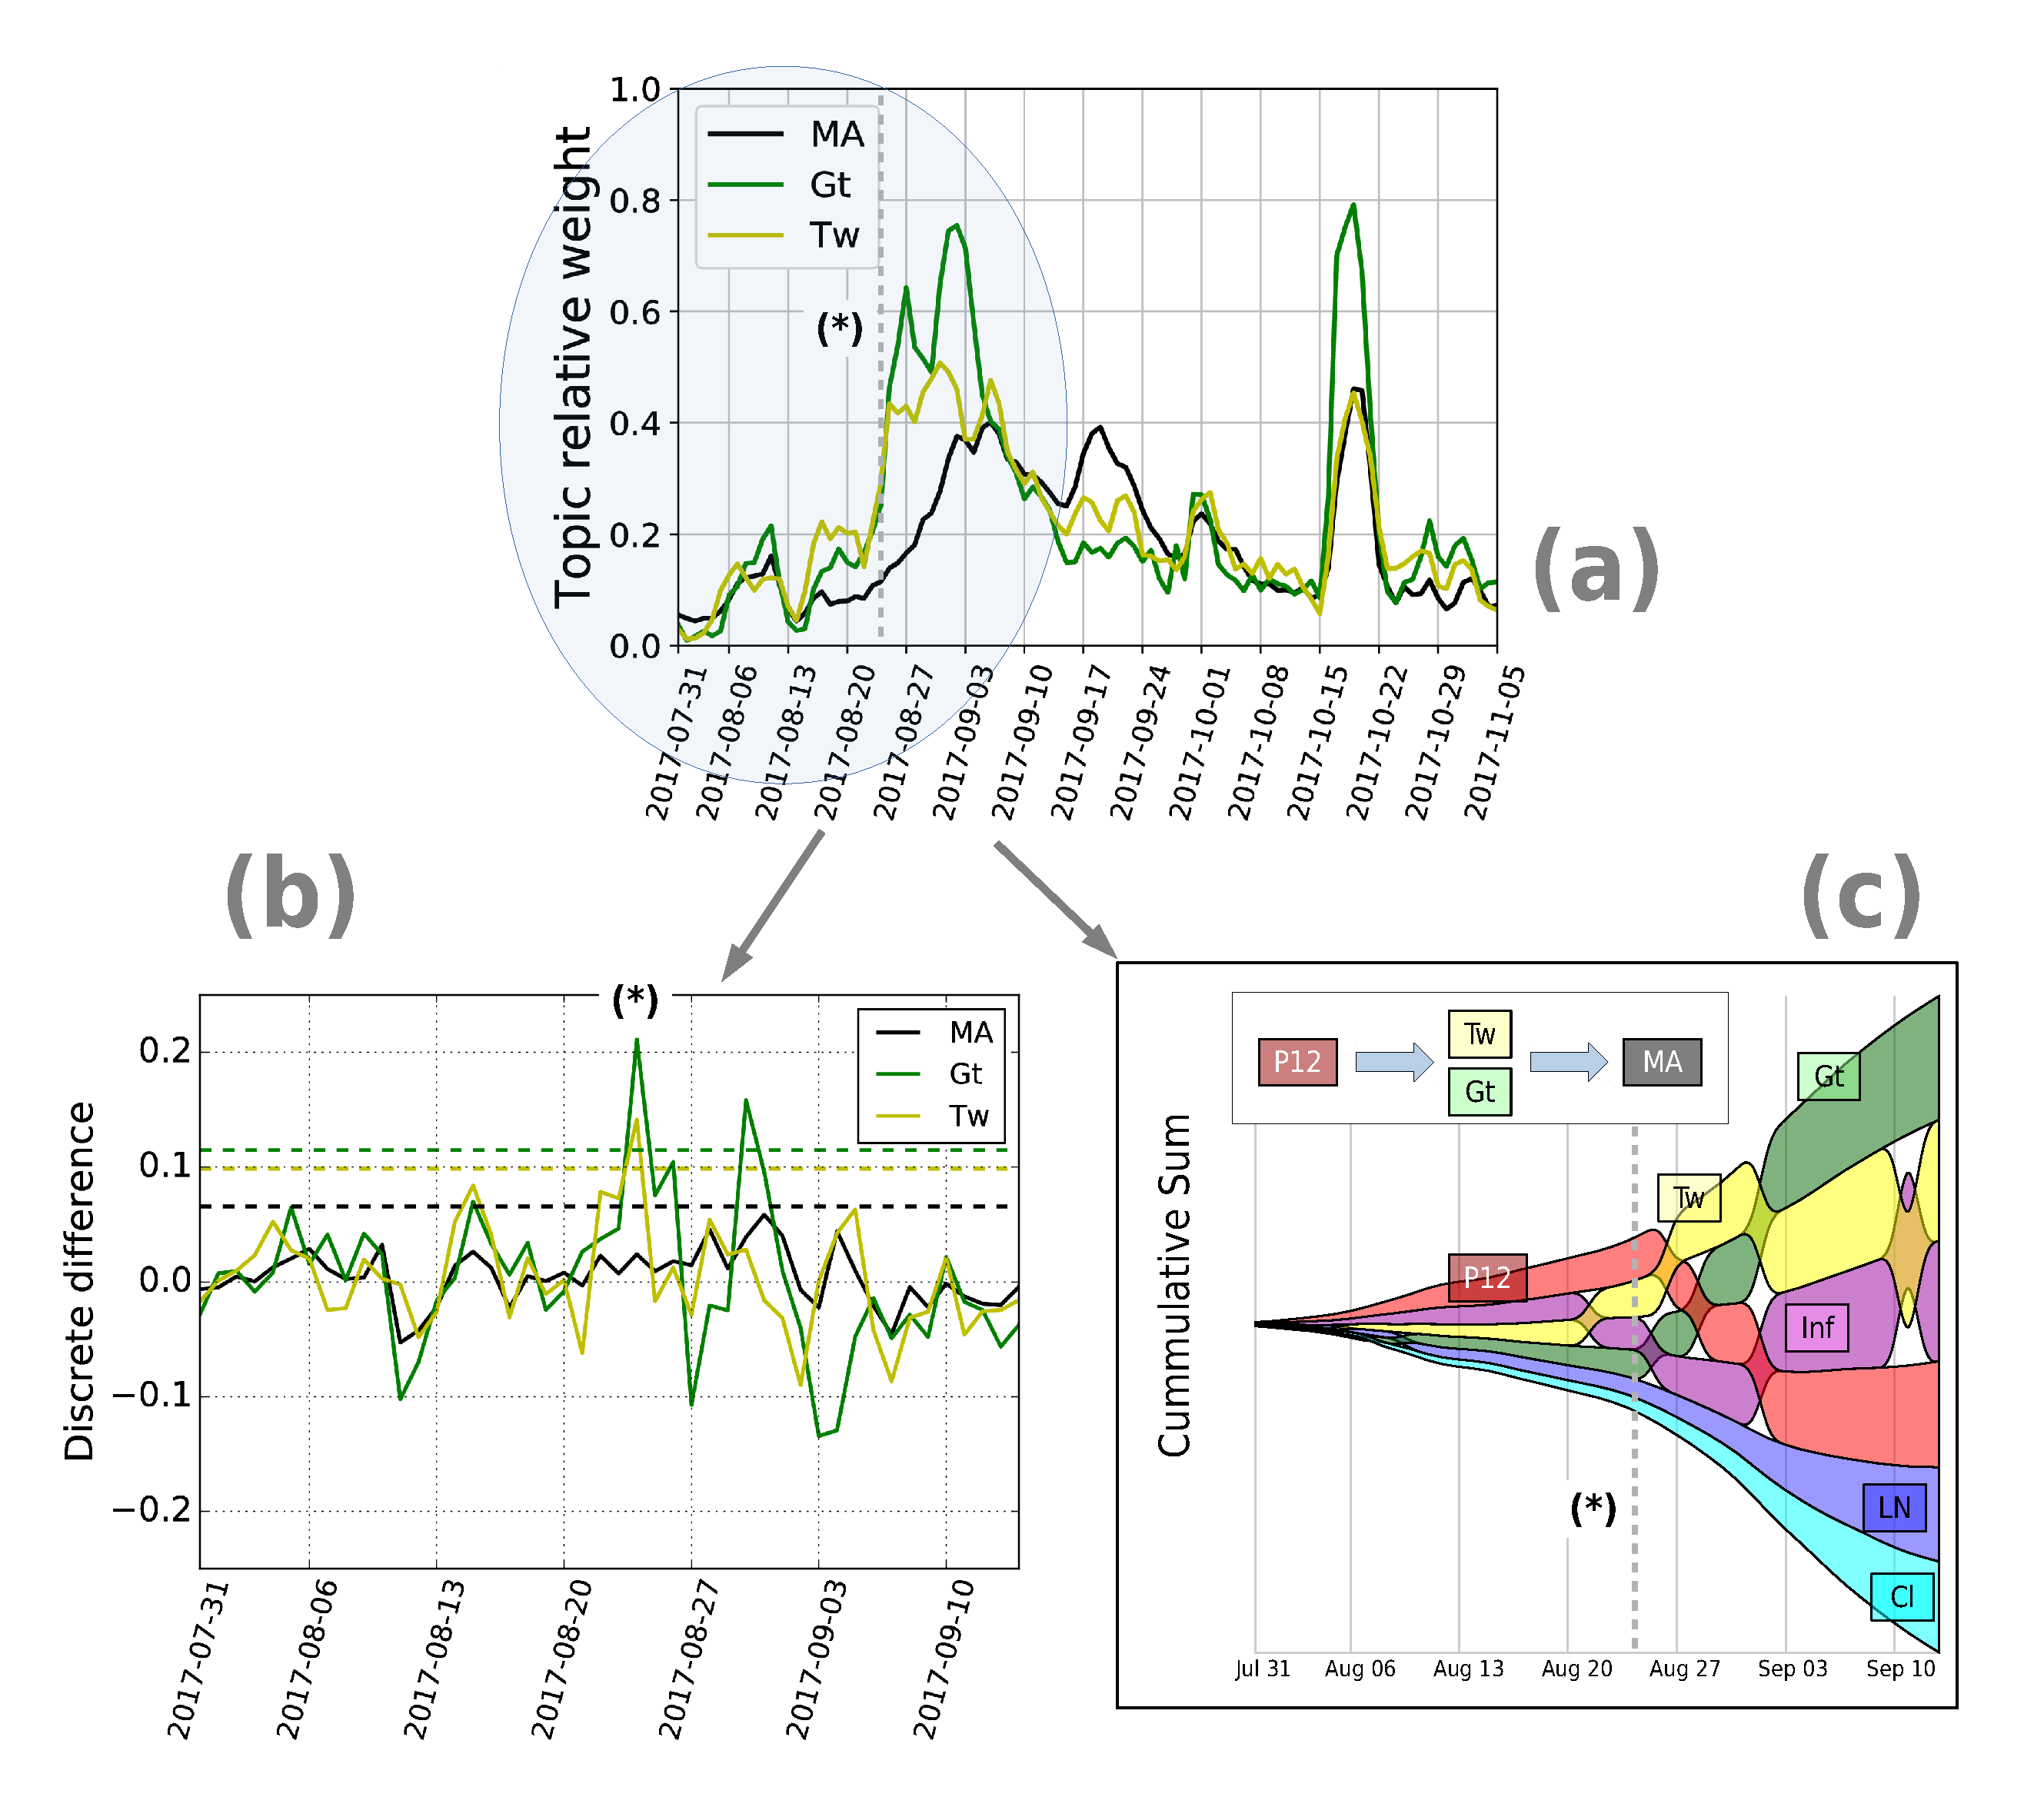
\includegraphics[width = \textwidth]{images/Fig8.pdf}
\caption{Agenda setting in Missing person's topic?}
\label{fig:Maldonado_setagenda}
\end{figure}




